\section{システム解析}
	前章で確定した線形モデルについてシステム解析を行う。これにより今回用いるモデル(上向きを基準とした線形状態方程式)が安定化制御可能か
	判定することができる。具体的には可制御性と可観測性を調べ、それらが存在すれば安定化制御可能であるといえる。
	以下で行う計算はすべて\MaTX{}を用いた。
	\subsection{安定性}
		システムの極($A$の固有値)を計算した結果$D$を以下に示す。
		\begin{equation}
			D=\left[
			\begin{array}{c}
				7.0\\
				0\\
				-6.8\\
				-11\\
			\end{array}
			\right]
			\label{eq:Aeig}
		\end{equation}
		(\ref{eq:Aeig})式より1行目が不安定であり、2行目が安定限界であるので、今回用いるモデルは
		不安定であるといえる。
	\subsection{可制御性}
		可制御性行列は以下のようになる。
		\[
			N_{c} = \left[
			\begin{array}{cccc}
				C & CA & CA^{2} & CA^{3} \\
			\end{array}
			\right]
		\]
		上の行列よりランクは4になれば可制御性があるといえる。ランクを計算したところ
		\[
			\rm{rank}  = 4
		\]
		となった。よって可制御性を確認できる。\\
	\subsection{可制御性}
		可観測性行列は以下のようになる。
		\[
			N_{o} = \left[
			\begin{array}{c}
				C\\
				CA\\
				CA^{2}\\
				CA^{3}\\
			\end{array}
			\right]
		\]
		上の行列よりランクは4になれば可観測性があるといえる。ランクを計算したところ
		\[
			\rm{rank} = 4
		\]
		となった。よって、可観測性を確認できる。\\
	\par
	以上から倒立振子系の上向き基準の線形モデルは不安定なシステムであるが、4つの状態を観測することができ、
	制御することが可能なシステムといえる。次の節では倒立振子を立たせるための制御器を設計していく。
	その際に前章で計算したシステム行列Aと入力行列Bを用いる。
		
%----------------------------------------------------------------------------------
\section{状態フィードバックの設計}
	制御器を設計していく第一段階として、状態フィードバック$F$の設計を行う。
	$F$は、システムを安定化する状態フィードバック
	\[
		u = -Fx
	\]
	として求めればよい。
	また、本実験においては台車が目標値へ移動を行うので、目標値$x_{ref}$
	として以下を設計することになる。
	\begin{equation}
		u(t) = F(x_{ref} - x)
		\label{eq:Feq1}
	\end{equation}
	% TODO←???
	この状態フィードバックの設計法には、極配置に基づく状態フィードバック測と
	LQ最適制御に基づく状態フィードバック測の2通りがあるが今回は後者の方法を用いて設計を行う。
	\par
	さて、(\ref{eq:Feq1})式をLQ問題の解として得るために、2次形式評価関数
	\begin{equation}
		J = \int_{0}^{\infty}(x^{T}Qx+Ru^{2})dt
		\label{eq:Feq2}
	\end{equation}
	\begin{equation}
		Q = \rm{diag}(q_{1}^2,q_{2}^2,q_{3}^2,q_{4}^2),\ \ R = 1
		\label{eq:Feq3}
	\end{equation}
	を考える。ただし、 $\rm{diag}(\ldots)$は、対角行列を表す。これは
	\begin{equation}
		J=\int_{0}^{\infty}(q_{1}^{2}r^{2}+q_{2}^{2}\theta^{2}
		+q_{3}^{2}\dot{r}^{2}+q_{4}^{2}\dot{\theta}^{2})dt
	\end{equation}
	のように表されることから、$q_1,q_2,q_3,q_4$は台車位置$r$、振り子角度$\theta$、
	台車速度$\dot{\theta}$、振子角速度$\dot{\theta}$の間のバランスをとる重み係数である。
	\par
	(\ref{eq:Feq2})と(\ref{eq:Feq3})式を最小にする(\ref{eq:Feq1})式における$F$は、
	リカッチの方程式
	\[
		A^{T}P+PA-PBR^{-1}B^{T}P+Q = 0
	\]
	の解$P>0$を求めて
	\[
		F = R^{-1}B^{T}P
	\]
	のように与えられる。
	\begin{figure}[h]
		\centering
		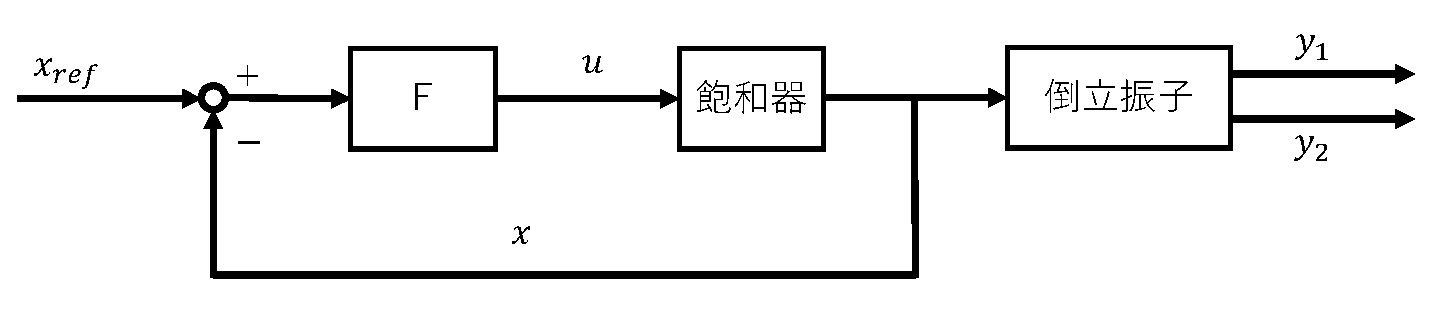
\includegraphics[width=0.8\linewidth]{gazo/controll_F.eps}
		\caption{状態フィードバックを含めたブロック線図}
		\label{image:cF}
	\end{figure}
%一次チェック完了
%----------------------------------------------------------------------------------
\section{最小次元オブザーバの設計}
	第二段階として、
	\begin{equation}
		\hat{x}→x\ \ (t→\infty)
		\label{eq:obs1}
	\end{equation}
	を満足させる状態を推定する状態観測器(最小次元オブザーバ)
	\begin{equation}
		\dot{z}(t) = \hat{A}z(t)+\hat{B}y(t)+\hat{J}u(t)
		\label{eq:obs2}
	\end{equation}
	\begin{equation}
		\hat{x}(t) = \hat{C}z(t) + \hat{D}y(t)
		\label{eq:obs3}
	\end{equation}
	をゴピナスの方法で設計する。
	この方法は、ある行列$U(1×4)$が存在して
	\[
		\begin{array}{c}
			UA = \hat{A}U + \hat{B}C \\
			UB = \hat{J}
			I = \hat{C}U + \hat{D}C
		\end{array}
	\]
	かつ$\hat{A}$が安定行列であることを満足する方法であり、オブザーバ(\ref{eq:obs2})、(\ref{eq:obs3})
	が(\ref{eq:obs1})式を満足するための十分条件でもある。
	なお、本実験で用いる倒立振子系は
	$r,\theta$はセンサーを用いて計測できるが、$\dot{r},\dot{\theta}$
	においては計測するためのセンサーが存在しないため、推測でしかこれらを得ることができない。
	その推測を行うのに、最小次元オブザーバーを用いる。
	\par
	具体的には、オブザーバの係数行列$\hat{A},\hat{B},\hat{J},\hat{C},\hat{D}$を求める。これらは適当な
	オブザーバの極を選択することで得ることができる。。
	また、オブザーバの極を決める際に、状態フィードバック制御
	\[
		u(t) = F(x_{ref}(t)-x(t))
	\]
	による閉ループ系
	\[
		\dot{x}(t) = (A-BF)x(t) + BFx_{ref}(t)
	\]
	の極との位置関係を考慮する必要がある。
	\begin{figure}[h]
		\centering
		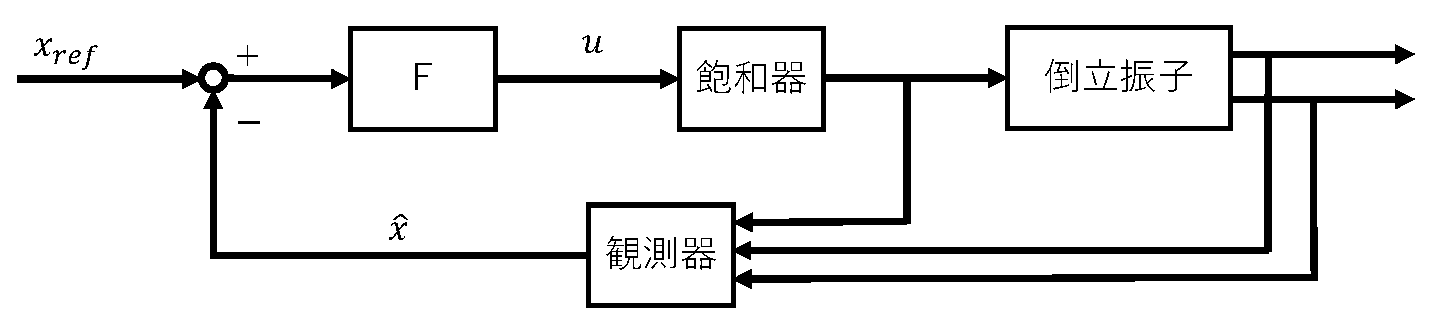
\includegraphics[width=0.8\linewidth]{gazo/controll_obs.eps}
		\caption{最小次元オブザーバーを含めたブロック線図}
		\label{image:cOBS}
	\end{figure}
%一次チェック完了
%----------------------------------------------------------------------------------
\section{コントローラの離散化}
	コントローラは連続時間で記述された(\ref{eq:Feq1})、(\ref{eq:obs2})、(\ref{eq:obs3})式
	で与えられるが、計算機制御のためにはこれらを離散時間で記述しなければならない。
	これらを離散化したものを離散時間コントローラと呼ぶ。離散時間コントローラは
	サンプリング周期を$\Delta$とすると、以下の式で与えられる。
	\begin{equation}
		z[k+1] = \hat{A}_{d}z[k]+\hat{B}_{d}y[k]+\hat{J}_{d}u[k]
	\end{equation}
	\begin{equation}
		\hat{x}[k] = \hat{C}_{d}z[k] + \hat{D}_{d}y[k]
	\end{equation}
	\begin{equation}
		u[k] = F(x_{ref}[k] - \hat{x}[k])
	\end{equation}
	ただし、$k = 0,1\ldots$であり
	\[
		\left(
		\begin{array}{cc}
			\hat{A}_{d} & [\hat{B}_{d}\ \hat{J}_{d}]\\
			0_{3×2} & I_{3}\\
		\end{array}
		\right)=\exp\left(\Delta\left(
		\begin{array}{cc}
			\hat{A} & [\hat{B}\ \hat{J}]\\
			0_{3×2} & I_{3}\\
		\end{array}
		\right)\right)
	\]
	である。
	具体的には、適当なサンプリング周期を$\Delta$を設定すればよい。
	\begin{figure}[h]
		\centering
		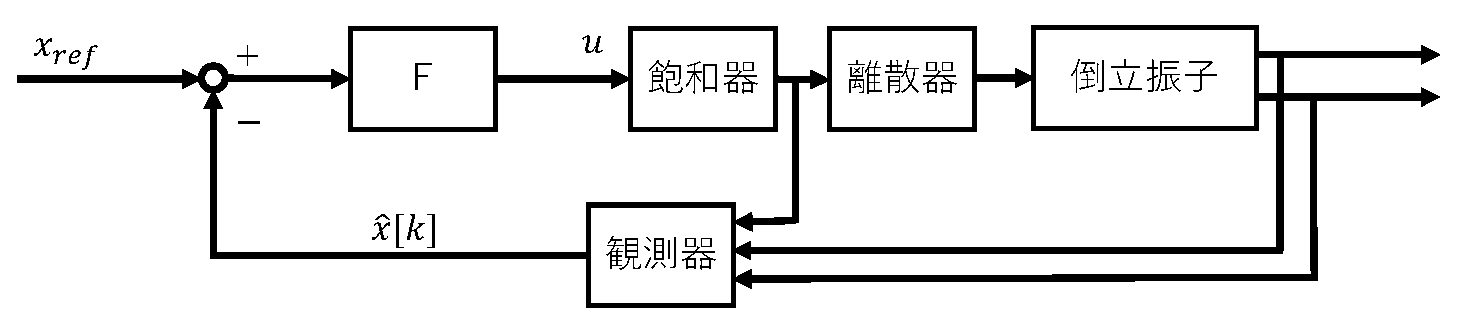
\includegraphics[width=0.8\linewidth]{gazo/controll_discrete.eps}
		\caption{離散器(0次ホールド)を含めたブロック線図}
		\label{image:cDISCRETE}
	\end{figure}
%一次チェック完了
%----------------------------------------------------------------------------------
\section{振り上げ制御及び安定化の実現}
	ここでは振子の振り上げ制御を行うためのコントローラを設計する。振り上げ制御とは、
	振り子を下向きにしたままで台車を動かすことで振り子を倒立させようという制御のことである。
	この制御には振り子を振り上げる制御と振り子の安定化制御を使い分けることで実現させる。
	具体的には下向きの振り子を振り上げ制御により徐々に上に持っていく($\theta$を0に近づけていく)、
	このときある一定の角度を境界値と定め、その境界値まで振り子の角度がちいさくなったところで制御を
	安定化制御に切り替え、安定化制御を行うというものである。振り子の安定化制御についてはこれまでのコントローラを用いるので、
	ここでは振り子の振り上げ制御の理論とその実現方法について述べる。
	\par
	台車と振り子の運動方程式は
	\begin{equation}
		(M+m)\ddot{r}+ml\cos{\theta}\ddot{\theta} = -f\dot{r} + ml\sin{\theta}\dot{\theta}^{2}+au\\
		\label{eq:huriage2}
	\end{equation}
	\begin{equation}
		ml\cos{\theta}\ddot{r}+(J+ml^{2})\ddot{\theta} = mgl\sin{\theta}-c\dot{\theta}\\
		\label{eq:huriage5}
	\end{equation}
	で与えられる。振り子が垂直上向きのときを基準とする振り子の力学的エネルギーは
	\[
		E = \frac{1}{2}(J+ml^{2})\dot{\theta}^{2}+mgl(\cos{\theta}-1)
	\]
	で与えられる。第一項が回転に関するエネルギーであり、第二項が傾きを考慮した位置エネルギーである。
	なお、基準において静止しているとき、力学的エネルギーはE=0である。
	このとき、力学的エネルギーの時間微分は
	\begin{equation}
		\frac{dE}{dt} = (J+ml)\dot{\theta}\ddot{\theta}-mgl\dot{\theta}\sin{\theta}
		\label{eq:huriage6}
	\end{equation}
	となる。振り上げ制御のために、次の制御則を用いる。
	\begin{equation}
		u = \frac{1}{a}\left(f\dot{r} - ml\sin{\theta}\dot{\theta}^{2} + ml\cos{\theta}\ddot{\theta} + (M+m)v \right)\\
		\label{eq:huriage1}
	\end{equation}
	\begin{equation}
		v = -\frac{c\dot{\theta}}{ml\cos{\theta}}+k(E-E_{0})\rm{sign}(\dot{\theta}\cos{\theta})
		\label{eq:huriage4}
	\end{equation}
	ただし、signは符合関数であり、引数の値が負のとき$-1$、正のとき1、0のとき0となる。
	(\ref{eq:huriage1})式を(\ref{eq:huriage2})式に代入すると、
	\begin{equation}
		\ddot{r} = v
		\label{eq:huriage3}
	\end{equation}
	を得る。(\ref{eq:huriage3})式と(\ref{eq:huriage4})式を(\ref{eq:huriage5})式に代入すると
	\[
		(J+ml^{2})\ddot{\theta} = mgl\sin{\theta}-ml\cos{\theta}(k(E-E_{0})\rm{sign}(\dot{\theta}\cos{\theta})
	\]
	を得る。この式を(\ref{eq:huriage6})式に代入すると
	\begin{align*}
			\displaystyle\frac{dE}{dt} &= -ml\dot{\theta}(k(E-E_{0})\rm{sign}(\dot{\theta}\cos{\theta})) \notag\\
			&= -mlk(E-E_{0})\rm{sign}(\dot{\theta}\cos{\theta})(\dot{\theta}\cos{\theta})
	\end{align*}
	となる。リアプノフ関数の候補として、
	\[
		V = \frac{(E-E_{0})^{2}}{2}≧0
	\]
	を考える。Vの時間微分を求めると、
	\begin{align*}
			\displaystyle \frac{dV}{dt} &= (E - E_{0})\frac{dE}{dt} \notag \\
			&= -mlk(E-E_{0})^{2}\rm{sign}(\dot{\theta}\cos{\theta})(\dot{\theta}\cos{\theta})≦0
	\end{align*}
	これより、$\dot{\theta}\cos{\theta}≠0$のとき、$\dot{V}<0$であるので$V$は減少して$0$に収束し、
	$E$は$E_0$に収束する。なお、$k$を大きくすると、早く$E$が$E_0$に収束する。
	実際の制御では、台車の加速度目標vを制限し、
	\begin{align}
			u &= \displaystyle\frac{1}{a}\left(f\dot{r} - ml\sin{\theta}\dot{\theta}^2 + ml\cos{\theta}\ddot{\theta}+(M+m)v \right) \notag\\
			v &= -\displaystyle\frac{c\dot{\theta}}{ml\cos{\theta}}+\rm{sat}_{ng}(k(E-E_{0})\rm{sign}(\dot{\theta}\cos{\theta}) \notag
	\end{align}
	とする。ただし、satは最小値が$-ng$,最大値が$ng$の飽和関数である。$n$は、重力加速度(鉛直下向き)
	と台車の加速度(水平方向)の比である。\\
	具体的には、$k$と重力加速度と台車の加速度の比である$n$を調整し、振り上げ制御を実現させる。
	\begin{figure}[H]
		\centering
		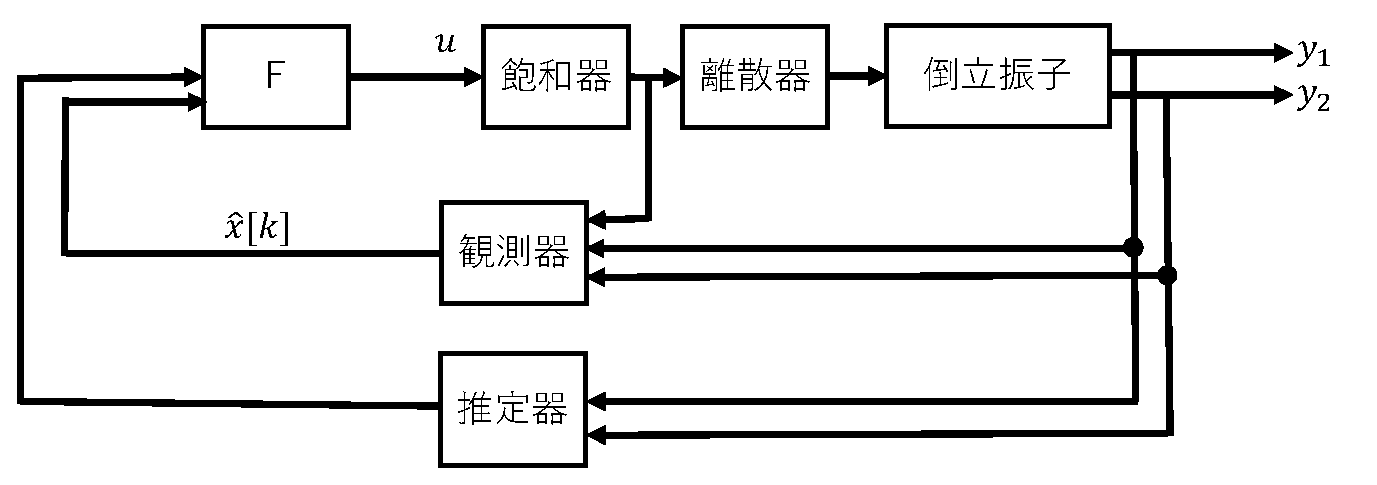
\includegraphics[width=0.8\linewidth]{gazo/controll_huriage.eps}
		\caption{振り上げ制御及び安定化制御を行うためのブロック線図}
		\label{image:cHURIAGE}
	\end{figure}
%一次チェック完了
%----------------------------------------------------------------------------------